% interactapasample.tex
% v1.05 - August 2017

\documentclass[]{interact}

\usepackage{minted} % for HaskellCode
\usepackage{epstopdf}% To incorporate .eps illustrations using PDFLaTeX, etc.
\usepackage[caption=false]{subfig}% Support for small, `sub' figures and tables
%\usepackage[nolists,tablesfirst]{endfloat}% To `separate' figures and tables from text if required
%\usepackage[doublespacing]{setspace}% To produce a `double spaced' document if required
%\setlength\parindent{24pt}% To increase paragraph indentation when line spacing is doubled

% UNCOMMENT WHEN USING BIBITEM
\usepackage[longnamesfirst,sort]{natbib}% Citation support using natbib.sty
\bibpunct[, ]{(}{)}{;}{a}{,}{,}% Citation support using natbib.sty
\renewcommand\bibfont{\fontsize{10}{12}\selectfont}% To set the list of references in 10 point font using natbib.sty

% define HaskellCode command for nice formatting of Haskell Code
\newminted[HaskellCode]{haskell}{fontsize=\footnotesize}

%\usepackage[natbibapa,nodoi]{apacite}% Citation support using apacite.sty. Commands using natbib.sty MUST be deactivated first!
%\setlength\bibhang{12pt}% To set the indentation in the list of references using apacite.sty. Commands using natbib.sty MUST be deactivated first!
%\renewcommand\bibliographytypesize{\fontsize{10}{12}\selectfont}% To set the list of references in 10 point font using apacite.sty. Commands using natbib.sty MUST be deactivated first!

\theoremstyle{plain}% Theorem-like structures provided by amsthm.sty
\newtheorem{theorem}{Theorem}[section]
\newtheorem{lemma}[theorem]{Lemma}
\newtheorem{corollary}[theorem]{Corollary}
\newtheorem{proposition}[theorem]{Proposition}

\theoremstyle{definition}
\newtheorem{definition}[theorem]{Definition}
\newtheorem{example}[theorem]{Example}

\theoremstyle{remark}
\newtheorem{remark}{Remark}
\newtheorem{notation}{Notation}

\begin{document}

\articletype{ARTICLE TEMPLATE}% Specify the article type or omit as appropriate

% 1. Author details. All authors of a manuscript should include their full name and affiliation on the cover page of the manuscript. Where available, please also include ORCiDs and social media handles (Facebook, Twitter or LinkedIn). One author will need to be identified as the corresponding author, with their email address normally displayed in the article PDF (depending on the journal) and the online article. Authors’ affiliations are the affiliations where the research was conducted. If any of the named co-authors moves affiliation during the peer-review process, the new affiliation can be given as a footnote. Please note that no changes to affiliation can be made after your paper is accepted. Read more on authorship.
\title{Specification Testing of Agent-Based Simulation using Property-Based Testing.}

\author{
\name{Jonathan Thaler \textsuperscript{a}\thanks{CONTACT Jonathan Thaler. Email: jonathan.thaler@nottingham.ac.uk} and Peer-Olaf Siebers\textsuperscript{a}}
\affil{\textsuperscript{a}School Of Computer Science, University of Nottingham, 7301 Wollaton Rd, Nottingham, UK;}
}



\maketitle

% 2. Should contain an unstructured abstract of 200 words. 
% 3. You can opt to include a video abstract with your article. Find out how these can help your work reach a wider audience, and what to think about when filming.
\begin{abstract}
This paper explores how to use random property-based testing on a technical level to encode and test specifications of agent-based simulations (ABS). The claim is that opposed to unit testing, random property-based testing is a much more natural fit to test ABS due to both stochastic nature. The paper shows how to test full agent- and model-specifications, in the case of an agents behaviour, its transition probabilities and model invariants. The outcome are specifications expressed directly in code, which relate whole classes of random input to expected classes of output. During test execution, random test data is generated automatically, potentially covering the equivalent of thousands of unit tests, run within seconds. The expressiveness and power of property-based testing is not only limited to be part of a test-driven development process where it acts as specification, verification and regression test but can be integrated as a fundamental part of the model development process, supporting the hypothesis and discovery making process. By incorporating this powerful technique into the simulation development process the confidence in the correctness of an implementation increases dramatically, something of fundamental importance for ABS in general and for ABS supporting far-reaching policy decisions in particular.
\end{abstract}

% 4. Between 3 and 6 keywords. Read making your article more discoverable, including information on choosing a title and search engine optimization.
\begin{keywords}
Testing; Test Driven Development; Model Specification;
\end{keywords}

% 5 Funding details - not required for this paper

% 6. Disclosure statement. This is to acknowledge any financial interest or benefit that has arisen from the direct applications of your research. - not required in this paper

% 7. Supplemental online material. Supplemental material can be a video, dataset, fileset, sound file or anything which supports (and is pertinent to) your paper. We publish supplemental material online via Figshare. 
% TODO

% 8. Figures. Figures should be high quality (1200 dpi for line art, 600 dpi for grayscale and 300 dpi for colour, at the correct size). Figures should be supplied in one of our preferred file formats: EPS, PS, JPEG, GIF, or Microsoft Word (DOC or DOCX). For information relating to other file types, please consult our Submission of electronic artwork document.

% 9. Tables. Tables should present new information rather than duplicating what is in the text. Readers should be able to interpret the table without reference to the text. Please supply editable files.

% 10. Equations. If you are submitting your manuscript as a Word document, please ensure that equations are editable. 

% 11. Units. Please use SI units (non-italicized).

% WORD LIMITS
% Please include a word count for your paper. A typical article for this journal should be no more than 6000 words; this limit does not include the abstract, endnotes, tables, figures, figure captions and legends, or references. 

\section{Introduction}
There exists a large number of simulation packages which allow the convenient creation of System Dynamics simulations by straight-forward visual diagram creation. One simply creates stocks and flows, connects them, specifies the flow-rates and initial parameters and then runs the model. An example for such a visual diagram creation in the simulation package AnyLogic can be seen in Figure \ref{fig:sir_stockflow_diagram}.

\begin{figure}
	\centering
	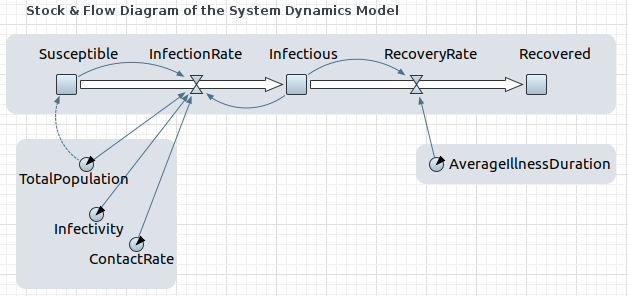
\includegraphics[width=.5\textwidth, angle=0]{./fig/SIR_SD_STOCKFLOW_DIAGRAMM.png}
	\caption{Visual System Dynamics Diagram of the SIR model in AnyLogic Personal Learning Edition 8.3.1.}
	\label{fig:sir_stockflow_diagram}
\end{figure}

Still, implementing System Dynamics directly in code is not as straight forward and involves numerical integration which can be quite tricky to get right. Thus, the aim of this paper is to look into how System Dynamics models can be implemented in code correctly without the use of a simulation package. We use the well known SIR model \cite{kermack_contribution_1927} from epidemiology to demonstrate our approach.

Our language of choice is Haskell because it emphasises a declarative programming style in which one describes \textit{what} instead of \textit{how} to compute. Further it allows to rule out interference with non-deterministic influences or side-effects already at compile-time. This is of fundamental importance for System Dynamics because it behaves completely deterministic and involves no stochastics or non-determinism whatsoever. Also, we make use of Functional Reactive Programming which allows to express continuous-time systems in a functional way. 

We show that by this approach we can arrive at correct-by-construction implementations of System Dynamic models. This means that the correctness of the code is obvious because we have closed the gap between the model specification and its implementation. Thus, the contribution of the paper is the demonstration of how to implement correct-by-construction System Dynamics simulations using Haskell and Functional Reactive Programming.

\section*{Property-Based Testing}
\label{sec:proptesting}

Property-based testing allows to formulate \textit{functional specifications} in code which then a property-based testing library tries to falsify by \textit{automatically} generating test-data, covering as much cases as possible. When a case is found for which the property fails, the library then reduces the test-data to its simplest form for which the test still fails e.g. shrinking a list to a smaller size. It is clear to see that this kind of testing is especially suited to ABS, because we can formulate specifications, meaning we describe \textit{what} to test instead of \textit{how} to test. Also the deductive nature of falsification in property-based testing suits very well the constructive and exploratory nature of ABS. Further, the automatic test-generation can make testing of large scenarios in ABS feasible because it does not require the programmer to specify all test-cases by hand, as is required in e.g. traditional unit tests.

Property-based testing was introduced in \cite{claessen_quickcheck_2000,claessen_testing_2002} where the authors present the QuickCheck library in Haskell, which tries to falsify the specifications by \textit{randomly} sampling the test space. We argue, that the stochastic sampling nature of this approach is particularly well suited to ABS, because it is itself almost always driven by stochastic events and randomness in the agents behaviour, thus this correlation should make it straightforward to map ABS to property-testing.
%The main challenge when using QuickCheck, as will be shown later, is to write \textit{custom} test-data generators for agents and the environment which cover the space sufficiently enough to not miss out on important test-cases.
According to the authors of QuickCheck \textit{"The major limitation is that there is no measurement of test coverage."} \cite{claessen_quickcheck_2000}. Although QuickCheck provides help to report the distribution of test-cases it is not able to measure the coverage of tests in general. This could lead to the case that test-cases which would fail are never tested because of the stochastic nature of QuickCheck. Fortunately, the library provides mechanisms for the developer to measure coverage in specific test-cases where the data and its (expected) distribution is known to the developer. This is a powerful tool for testing randomness in ABS as will be shown in subsequent chapters.

\medskip

As a remedy for the potential coverage problems of QuickCheck, there exists also a deterministic property-testing library called SmallCheck \cite{runciman_smallcheck_2008}, which instead of randomly sampling the test-space, enumerates test-cases exhaustively up to some depth. It is based on two observations, derived from model-checking, that (1) \textit{"If a program fails to meet its specification in some cases, it almost always fails in some simple case"} and (2) \textit{"If a program does not fail in any simple case, it hardly ever fails in any case} \cite{runciman_smallcheck_2008}. This non-stochastic approach to property-based testing might be a complementary addition in some cases where the tests are of non-stochastic nature with a search-space  too large to test manually by unit tests but small enough to enumerate exhaustively. The main difficulty and weakness of using SmallCheck is to reduce the dimensionality of the test-case depth search to prevent combinatorial explosion, which would lead to exponential number of cases. Thus one can see QuickCheck and SmallCheck as complementary instead of in opposition to each other.

\subsection*{A brief overview of QuickCheck}
To give a rough idea on how property-based testing works in Haskell, we give a few examples of property-tests on lists, which are directly expressed as functions in Haskell. Such a function has to return a \textit{Bool} which indicates \textit{True} in case the test succeeds or \textit{False} if not and can take input arguments which data is automatically generated by QuickCheck.

\begin{HaskellCode}
-- concatenation operator (++) is associative
append_associative :: [Int] -> [Int] -> [Int] -> Bool
append_associative xs ys zs = (xs ++ ys) ++ zs == xs ++ (ys ++ zs)

-- the reverse of a reversed list is the original list
reverse_reverse :: [Int] -> Bool
reverse_reverse xs = reverse (reverse xs) == xs

-- reverse is distributive over concatenation (++)
-- this test fails for explanatory reasons, for a correct 
-- property xs and ys need to be swapped on the right-hand side!
reverse_distributive :: [Int] -> [Int] -> Bool
reverse_distributive xs ys = reverse (xs ++ ys) == reverse xs ++ reverse ys

-- running the tests
main :: IO ()
main = do
  quickCheck append_associative
  quickCheck reverse_reverse
  quickCheck reverse_distributive
\end{HaskellCode}

When we run the tests using \textit{main}, we get the following output:

\begin{verbatim}
+++ OK, passed 100 tests.
+++ OK, passed 100 tests.
*** Failed! Falsifiable (after 5 tests and 6 shrinks):    
[0]
[1]
\end{verbatim}

We see that QuickCheck generates 100 test-cases for each property-test and it does this by generating random data for the input arguments. Note that we have not specified any data for our input arguments; QuickCheck is able to provide a suitable data-generator through type-inference: for lists and all the existing Haskell types like Int there exist custom generators already.

QuickCheck generates 100 test-cases by default and requires all to pass - if there is a test-case which fails, the overall property-test fails and QuickCheck shrinks the input to a minimal size for which the case still fails and reports it as a counter example. This is the case in the last property-test \textit{reverse\_distributive} which is wrong as \textit{xs} and \textit{ys} need to be swapped on the right-hand side. In this run, QuickCheck found a counter-example to the property after 5 tests and applied 6 shrinks to find the minimal failing example of \textit{xs = [0]} and \textit{ys = [1]}. If we swap \textit{xs} and \textit{ys}, the property-test passes 100 test-cases just like the other two did. Note that it is possible to configure QuickCheck to generate more or less random test-cases, which can be used to increase the coverage if the sampling space is quite large - this will become useful later.

\subsubsection*{Properties and Generators}
TODO: property
TODO: label
TODO: ==>
TODO: generators

\subsubsection*{Coverage}
TODO: cover with checkCoverage


\chapter{Conclusions}
\label{chap:concl}

\section{Being Realistic}
It is of most importance to stress that we don't condemn the current state-of-the-art approach of object-oriented specification and implementation to ABS. The strength of object-oriented programming is surely that it can be seen as \textit{programming as modelling} and thus will be always an attractive approach to ABS. Also we are realists and know that there are more points to consider when selecting a set of methods for developing software for an ABS than robustness, verification and validation. Almost always the popularity of an existing language and which languages the implementer knows is the driving force behind which methods and languages to choose. This means that ABS will continue to be implemented in object-oriented programming languages and many perfectly well functioning models will be created by it in the future. Although they all suffer from the same issues mentioned in the introduction this doesn't matter as they are not of central importance to most of them.
Nonetheless we think our work is still essential and necessary as it may start a slow paradigm-shift and opens up the minds of the ABS community to a more functional and formal way of approaching and implementing agent-based models and simulations and recognizing the benefits one gets automatically from it by doing so.

\section{What we are not doing}
Because of this highly interdisciplinary topic we explicitly mention what we do not want to undertake in this PhD.
First we don't want to develop another language for formal agent-specification which needs to be compiled or used in some fancy tool - we want to put it directly into Haskell, building on the existing facilities.
Second, we are not developing a new economic theory about decentralized bilateral bartering, we take the existing theory and existing agent-based models and apply our methods to them.
Third, we don't want to use fancy statistics and number juggling for comparing validating and verifying models: we want structural comparison (category-theory).
Fourth, we do NOT want to do a direct comparison of object-orientation vs. functional in ABS, as we would get lost in an infinite amount of low-level technical details. We look at the benefits / drawbacks more on a conceptual level, applied to ABS.

% TODO bibliography, only copy the references really cited in this paper, otherwise ALL will be included. then fix it
\input{references_bibitem}
%\bibliographystyle{acm}
\bibliographystyle{apacite}
\bibliography{references}

\end{document}